\documentclass[aspectratio=54,10pt,xcolor=x11names]{beamer}
  \usepackage[francais]{babel}
  \usepackage[autolanguage]{numprint}
  \usepackage{amsmath,icomma}
  \usepackage{booktabs,tabularx}
  \usepackage{pgfpages}
  \usepackage{metalogo}                % \XeLaTeX logo
  \usepackage{fontawesome}
  \usepackage{listings}
  \usepackage[overlay,absolute]{textpos}

  %%% Polices de caractères
  \usepackage{fontspec}
  \usepackage{unicode-math}
  \defaultfontfeatures{Ligatures=TeX}
  \setmainfont{Lucida Bright OT}
  \setsansfont{Lucida Sans OT}
  \setmathfont{Lucida Bright Math OT}
  \setmonofont[Scale=0.95]{Bitstream Vera Sans Mono}
  \newfontfamily\titles{Myriad Pro}
  \usepackage{microtype}

  %% Définition de nouveaux symboles de la police Font Awesome pas
  %% encore définis dans le package fontawesome (v. 3.1.1)
  \def\faFileText{{\FA \symbol{"F0F6}}}
  \def\faFilePDF{{\FA \symbol{"F1C1}}}
  \def\faYouTubePlay{{\FA \symbol{"F16A}}}

  %%% Titre
  \title[]{Rédaction de thèses et de mémoire avec {\LaTeX}: premiers pas}
  \author[]{Université Laval}
  \date{}
  \renewcommand{\year}{2015}    % pour notice de copyright

  %%% Définition de couleurs
  \definecolor{comments}{rgb}{0.7,0,0}
  \definecolor{alert}{rgb}{0,0.7,0}
  \definecolor{emphasis}{named}{orange}
  \definecolor{exercices}{named}{gray}
  \definecolor{link}{rgb}{0,0.4,0.6}   % ~RoyalBlue de dvips
  \definecolor{url}{rgb}{0.6,0,0}      % rouge-brun
  \hypersetup{colorlinks,allcolors=emphasis,urlcolor=url}

  %%% Paramètres de beamer
  \useinnertheme{default}
  \useoutertheme[width=10mm,height=2.2\baselineskip]{sidebar}
  \usefonttheme[onlylarge]{structurebold}
  \usefonttheme{professionalfonts}
  \addtobeamertemplate{headline}{\rule{0pt}{12pt}\par}{}
  \setbeamercolor{frametitle}{fg=white,bg=black}
  \setbeamerfont{frametitle}{family=\titles}
  \setbeamercolor{structure}{fg=emphasis,bg=white}
  \setbeamercolor{block title}{fg=white,bg=black}
  \setbeamercolor{alerted text}{fg=black}
  \setbeamerfont{alerted text}{series=\bfseries}
  \setbeamercolor{block title alerted}{fg=white,bg=alert}
  \setbeamercolor{block title example}{fg=white,bg=exercices}
  \setbeamercolor{example text}{fg=exercices,bg=white}
  \setbeamertemplate{theorems}[numbered]
  \setbeamertemplate{section in toc}[sections numbered]
  \setbeamertemplate{navigation symbols}{}
  \setbeamertemplate{section in sidebar}{}
  \setbeamertemplate{section in sidebar shaded}{}
  \AtBeginSection[]
  {
    \begin{frame}
      \frametitle{Sommaire}
      \small\tableofcontents[currentsection]
    \end{frame}
  }

  %%% Nouvelles commandes et nouveaux environnements
  \newcommand{\fichier}[1]{\texttt{#1}}
  \newcommand{\class}[1]{\textbf{#1}}
  \newcommand{\pkg}[1]{\textbf{#1}}

  \renewenvironment{quote}{%
    \begin{beamercolorbox}[wd=\linewidth,sep=6pt]{block body example}}
    {\end{beamercolorbox}}
  \newenvironment{texoutput}[1]{%
    \begin{minipage}[t]{#1} \small}{%
    \end{minipage}}
  \newenvironment{conseil}{%
    \begin{minipage}[t]{0.1\textwidth}
      \color{alert}\raisebox{-2.3em}[0em][0em]{\huge\faThumbsUp}
    \end{minipage}
    \begin{minipage}[t]{0.8\textwidth}
      \begin{alertblock}{Conseil du {\TeX}pert}}{%
    \end{alertblock}
    \end{minipage}}

  \theoremstyle{example}
  \newtheorem{exercice}[theorem]{Exercice}

  %%% Paramètres de listings
  \lstloadlanguages{[LaTeX]TeX}
  \lstset{language=[LaTeX]TeX,
    escapeinside=`',
    extendedchars=true,
    inputencoding=utf8/latin1,
    basicstyle=\small\ttfamily\NoAutoSpacing,
    commentstyle=\color{comments}\slshape,
    keywordstyle=\mdseries,
    emphstyle=\color{emphasis}\bfseries,
    backgroundcolor=\color{LightYellow1},
    frame=none,
    showstringspaces=false}

\begin{document}

%% Le code de la page couverture est conservé dans un fichier séparé
%% Avec l'option aspectratio=54, la taille des diapos est 125mm x 100mm

\begin{textblock*}{100mm}(-8mm,29mm)
  
\includegraphics[width=100mm,keepaspectratio]{TeXFZoneColor}
\end{textblock*}

\begin{textblock*}{107mm}(0mm,10mm)
  \rule[0mm]{107mm}{13mm}
\end{textblock*}

\begin{textblock*}{98mm}(7mm,14mm)
  \color{white}\fontspec{Myriad Pro}
  \fontsize{17pt}{18pt}\selectfont\bfseries%
  Rédaction de thèses et de mémoires
\end{textblock*}

\begin{textblock*}{70mm}(55mm,32mm)
  \color{black}\fontspec{Lucida Bright OT}
  \fontsize{17pt}{18pt}\selectfont%
  avec\;\;
  \fontsize{60pt}{60pt}\selectfont%
  \raisebox{-1.07ex}{\LaTeX}
\end{textblock*}

\begin{textblock*}{30mm}(85mm,63mm)
  \fontspec{Myriad Pro}
  \small\bfseries%
  1. PREMIERS PAS
\end{textblock*}

\begin{textblock*}{25mm}(93.5mm,80mm)
  
\includegraphics[width=25mm,keepaspectratio]{ul_p}
\end{textblock*}


%% Le texte du contrat de licence est conservé dans un fichier séparé
%%% Texte du contrat de licence au début des diapos

\begin{frame}[t,plain]
  \tiny
  \vspace*{10mm}

  {\textcopyright} {\year} Vincent Goulet, Université Laval \\[4mm]

  
\includegraphics[height=4mm,keepaspectratio=true]{by-sa} \\%

  Cette création est mise à disposition selon le contrat
  \href{http://creativecommons.org/licenses/by-sa/4.0/deed.fr}{%
    Attribution-Partage dans les mêmes conditions 4.0 International}
  de Creative Commons. En vertu de ce contrat, vous êtes libre de:
  \begin{itemize}
  \item[\color{black}\tiny$\blacktriangleright$]%
    \textbf{partager} --- reproduire, distribuer et communiquer
    l'{\oe}uvre;
  \item[\color{black}\tiny$\blacktriangleright$]%
    \textbf{remixer} --- adapter l'{\oe}uvre;
  \item[\color{black}\tiny$\blacktriangleright$]
    utiliser cette {\oe}uvre à des fins commerciales.
  \end{itemize}
  Selon les conditions suivantes:
  \vspace*{2mm}

  \begin{tabularx}{\linewidth}{@{}lX@{}}
    \raisebox{-5.5mm}[0mm][10mm]{%
      
\includegraphics[height=7mm,keepaspectratio=true]{by}}
    & \textbf{Attribution} --- Vous devez créditer l'{\oe}uvre, intégrer
      un lien vers le contrat et indiquer si des modifications ont été
      effectuées à l'{\oe}uvre. Vous devez indiquer ces informations par
      tous les moyens possibles, mais vous ne pouvez suggérer que
      l'Offrant vous soutient ou soutient la façon dont vous avez
      utilisé son {\oe}uvre. \\
    \raisebox{-5.5mm}{
\includegraphics[height=7mm,keepaspectratio=true]{sa}}
    & \textbf{Partage dans les mêmes conditions} --- Dans le cas où
      vous modifiez, transformez ou créez à partir du matériel composant
      l'{\oe}uvre originale, vous devez diffuser l'{\oe}uvre modifiée
      dans les même conditions, c'est à dire avec le même contrat avec
      lequel l'{\oe}uvre originale a été diffusée.
  \end{tabularx}
  \vspace*{4mm}

  Notes de cours et exercices développés par Vincent Goulet avec la
  contribution financière de la Bibliothèque de l'Université Laval.
  \vfill

  ISBN {\ISBN} \\
  Dépôt légal -- Bibliothèque et Archives nationales du Québec, {\year} \\
  Dépôt légal -- Bibliothèque et Archives Canada, {\year}
  \vfill

  \begin{minipage}{0.55\textwidth}
    \begin{tabularx}{\linewidth}{@{}Xl@{}}
      \textbf{Code source} \\
      Le code source de ce document est conservé dans un dépôt
      Subversion public. &
                           \raisebox{-3pt}{%
                           \href{https://svn.fsg.ulaval.ca/svn-pub/vgoulet/formation_latex/}{%
                           \browsebutton}}
    \end{tabularx}
  \end{minipage}
  \hfill
  \begin{minipage}{0.4\textwidth}
    \begin{tabularx}{\linewidth}{@{}X@{}}
      \textbf{Crédits} \\
      Couverture réalisée par Marie-Ève Guérard et \newline Hélène
      Coulouarn. Lion de CTAN réalisé par Duane Bibby.
    \end{tabularx}
  \end{minipage}
  \vfill

\end{frame}

%%% Local Variables:
%%% mode: latex
%%% TeX-master: "formation_latex-partie_1"
%%% coding: utf-8
%%% End:


\begin{frame}
  \frametitle{Sommaire}
  \small\tableofcontents
\end{frame}

\begin{frame}
  \frametitle{Pré-requis à cette formation}
  \begin{enumerate}
  \item Installer une distribution {\LaTeX} sur votre poste de
    travail; nous recommandons la distribution {\TeX}~Live
    \begin{itemize}
    \item[] \href{https://www.youtube.com/watch?v=fjcR6lFy0c4}{%
        {\faYouTubePlay} installation sur Mac OS X}
    \item[] \href{https://www.youtube.com/watch?v=z_dq3dns-WU}{%
        {\faYouTubePlay} installation sur Windows}
    \end{itemize}
    \bigskip
  \item Compiler un premier très simple de type \emph{Hello World!}
    \begin{itemize}
    \item[] \href{https://www.youtube.com/watch?v=QOUx_aOZ42o}{%
        {\faYouTubePlay} démonstration sur Mac OS X avec TeXShop}
    \item[] \href{https://www.youtube.com/watch?v=qddRMGwXnNM}{%
        {\faYouTubePlay} démonstration sur Windows avec Texmaker}
    \end{itemize}
  \end{enumerate}
\end{frame}


\section{{\TeX}, {\LaTeX} et consorts: ce que c'est et ce que ce n'est pas}

\begin{frame}
  \frametitle{Ce que c'est}
  \begin{itemize}
  \item Un système de mise en page (\emph{typesetting}) ou de préparation de
    documents
  \item {\LaTeX} est un ensemble de macro commandes pour faciliter
    l'utilisation de {\TeX}
  \item Langage de balisage (\emph{Markup Language}) pour indiquer la
    mise en forme du texte
  \item Accent mis sur la production de documents de grande qualité à
    la typographie soignée (surtout pour les mathématiques)
  \end{itemize}
\end{frame}

\begin{frame}
  \frametitle{Exemples de typographie soignée}
  \begin{itemize}
  \item Ligatures
    \begin{quote}
      \begin{minipage}{0.45\linewidth}
        \vspace{-12pt}
        \begin{block}{\small Word}
          \rmfamily f\/f \quad f\/i \quad f\/l \quad f\/f\/i \quad
          f\/f\/l
        \end{block}
      \end{minipage}
      \hfill
      \begin{minipage}{0.4\linewidth}
        \vspace{-12pt}
        \begin{block}{\small \LaTeX}
          \rmfamily ff \quad fi \quad fl \quad ffi \quad ffl
        \end{block}
      \end{minipage}
    \end{quote}
  \item Espacement des lettres
    \begin{quote}
      \begin{minipage}{0.45\linewidth}
        \vspace{-12pt}
        \begin{block}{\small texte}
          \rmfamily xy \quad \emph{xy}
        \end{block}
      \end{minipage}
      \hfill
      \begin{minipage}{0.4\linewidth}
        \vspace{-12pt}
        \begin{block}{\small mathématiques}
          $xy$
        \end{block}
      \end{minipage}
    \end{quote}
  \end{itemize}
\end{frame}

\begin{frame}
  \frametitle{Ce que ce n'est pas}
  \begin{itemize}
  \item Un traitement de texte
  \item WYSIWYG
  \item Incompatible
  \item Instable
  \item Imprévisible
  \end{itemize}
\end{frame}

\begin{frame}
  \frametitle{Processus de création d'un document {\LaTeX}}
  \Huge
  \begin{minipage}[t]{0.25\linewidth}
    \centering
    \faFileText \\ \bigskip
    \footnotesize
    rédaction du texte et balisage avec un \emph{éditeur de texte}
  \end{minipage}
  \hfill\faArrowRight\hfill
  \begin{minipage}[t]{0.25\linewidth}
    \centering
    \faCogs \\  \bigskip
    \footnotesize
    compilation avec un \emph{moteur} {\TeX} depuis la ligne de commande
  \end{minipage}
  \hfill\faArrowRight\hfill
  \begin{minipage}[t]{0.25\linewidth}
    \centering
    \faFilePDF \\  \bigskip
    \footnotesize
    visualisation avec visionneuse externe (Aperçu,
    SumatraPDF, etc.)
  \end{minipage}
  \newline\pause
  \begin{picture}(0,0)
    \thicklines\color{blue}
    \put(-5,-2){\dashbox{2}(200,100){}}
    \put(45,-5){
      \begin{minipage}[t]{105\unitlength}
        \footnotesize\centering
        \mbox{} \\ facilité par l'utilisation
        d'un logiciel intégré de rédaction
      \end{minipage}}
  \end{picture}
\end{frame}

%%% >>>
\begin{frame}[plain,fragile=singleslide]
  \begin{exercice}
    \begin{enumerate}
    \item Démarrer le logiciel Texmaker (ou tout autre
      éditeur ou logiciel intégré de rédaction de votre choix).
    \item Ouvrir et compiler le fichier \fichier{exercice\_minimal.tex}.
    \end{enumerate}
  \end{exercice}
\end{frame}
%%% <<<


\begin{frame}
  \frametitle{Quelques choses simples à réaliser avec {\LaTeX}}
  \framesubtitle{(et pas nécessairement avec un traitement de texte)}
  \begin{itemize}
  \item Page titre
  \item Table des matières
  \item Numérotation des pages
  \item Numérotation des équations et renvois
  \item Bibliographie et renvois
  \item Figures et tableaux: disposition sur la page, numérotation, renvois
  \item Coupure de mots
  \item Document recto-verso
  \end{itemize}
\end{frame}

\begin{frame}
  \frametitle{Moteurs et formats}
  \begin{tabular}{r}
    \\ \addlinespace[8pt] \\ \\
    \color{emphasis}\faArrowRight \\
    \color{emphasis}\faArrowRight
  \end{tabular}
  \hspace{-5mm}
  \begin{tabularx}{0.9\linewidth}{Xlc}
    \toprule[2pt]
    Moteur & Format & Fichier de sortie \\
    \midrule
    \texttt{tex} & plain \TeX & DVI \\
    \texttt{tex} (\texttt{latex}) & \LaTeX & DVI \\
    \texttt{pdftex} (\texttt{pdflatex}) & pdf\LaTeX & PDF \\
    \texttt{xetex} (\texttt{xelatex}) & \XeLaTeX & PDF \\
    \bottomrule[2pt]
  \end{tabularx}
\end{frame}

\begin{frame}
  \frametitle{Distributions}

  Le système {\LaTeX} est rendu disponible sous forme de \emph{distributions}

  \begin{itemize}
  \item Windows: {\TeX}~Live et MiK{\TeX}
  \item OS~X: Mac{\TeX} (dérivée de {\TeX}~Live)
  \item Linux: {\TeX}~Live
  \end{itemize}
  La Bibliothèque et la Faculté des études supérieures et
  post-doctorales recommandent {\TeX}~Live
\end{frame}

\begin{frame}[fragile=singleslide]
  \frametitle{Faits amusants}
  \begin{itemize}
  \item {\TeX} est aujourd'hui considéré essentiellement exempt de bogue
  \item Récompense si vous en trouvez un!
  \item Numéro de version de {\TeX} converge vers $\pi$:
\begin{lstlisting}
$ tex --version
TeX `\textbf{3.14159265}' (TeX Live 2014)
kpathsea version 6.2.0
Copyright 2014 D.E. Knuth.
[...]
\end{lstlisting}
  \item Pour en savoir plus:
    \begin{itemize}
    \item \href{http://www.tug.org/whatis.html}{Histoire de \TeX} (anglais)
    \item {\TeX} sur Wikipedia
      (\href{http://fr.wikipedia.org/wiki/TeX}{français};
      \href{http://en.wikipedia.org/wiki/TeX}{anglais}, plus complet)
    \end{itemize}
  \end{itemize}
\end{frame}


\section{Principes de base}

\begin{frame}[fragile=singleslide]
  \frametitle{Rédaction}
  \begin{itemize}
  \item On se concentre sur le contenu et la \alert{structure} du
    document, pas sur son \alert{apparence}
      \bigskip
      \begin{tabbing}
        \verb=\textbf{titre}= \qquad\= \faArrowRight \qquad\= \verb|\section{titre}| \\[6pt]
        \verb|\textit{texte}| \> \faArrowRight \> \verb|\emph{texte}|
      \end{tabbing}
      \bigskip
  \item Apparence prise en charge par {\LaTeX} et généralement préférable de ne
    pas la modifier
  \item Mots séparés par une ou plusieurs \alert{espaces}
  \item Paragraphes séparés par une ou plusieurs \alert{lignes blanches}
  \item Utilisation de \alert{commandes} pour indiquer la structure du texte
  \end{itemize}
\end{frame}

\begin{frame}[fragile=singleslide]
  \frametitle{Structure d'un document {\LaTeX}}
  Un fichier source {\LaTeX} est toujours composé de deux
  parties:
  \begin{enumerate}
  \item le \alert{préambule}
    \begin{itemize}
    \item suite de commandes spécifiant la mise en forme \emph{globale} du
      document (format du papier, marges, entête et pied de page, etc.)
    \item au minimum \verb=\documentclass=
    \end{itemize}
  \item le \alert{corps} du document
    \begin{itemize}
    \item débute par \verb=\begin{document}=
    \item texte du document
    \item commandes à effet \emph{local}
    \item termine par \verb=\end{document}=
    \end{itemize}
  \end{enumerate}
\end{frame}

%%% >>>
\begin{frame}[plain,fragile=singleslide]
  \begin{exercice}
    Utiliser le fichier \fichier{exercice\_minimal.tex}.
    \begin{enumerate}
    \item Compiler le document avec la classe \class{article}, puis
      avec la classe \class{book}. Observer le résultat.
    \item Ajouter du texte en français (avec accents) et observer le
      résultat.
    \item Question de voir ce que {\LaTeX} peut faire, compiler le
      document élaboré \fichier{exercice\_demo.tex} de la manière suivante:
      \begin{enumerate}[i)]
      \item une fois avec \texttt{LaTeX};
      \item une fois avec \texttt{BibTeX};
      \item deux à trois fois avec \texttt{LaTeX}.
      \end{enumerate}
    \end{enumerate}
  \end{exercice}
\end{frame}
%%% <<<

\begin{frame}[fragile=singleslide]
  \frametitle{Commandes}
  \begin{itemize}
  \item Débutent toujours par \verb=\=
  \item Nom se termine par tout caractère qui n'est pas une lettre (y
    compris l'espace!)
  \item Arguments obligatoires entre \verb={ }=
  \item Arguments optionnels entre \verb=[ ]=
  \item Formes générales:
\begin{lstlisting}
\`\textit{nomcommande}'[`\textit{arg\_optionnel}']{`\textit{arg\_obligatoire}'}
\`\textit{nomcommande}'*[`\textit{arg\_optionnel}']{`\textit{arg\_obligatoire}'}
\end{lstlisting}
  \item Portée d'une commande limitée à la zone entre \verb={ }=
  \end{itemize}
\end{frame}

\begin{frame}[fragile=singleslide]
  \frametitle{Environnements}
  \begin{itemize}
  \item Délimités par
\begin{lstlisting}
\begin{`\textit{environnement}'}

\end{`\textit{environnement}'}
    \end{lstlisting}
  \item Contenu de l'environnement traité différemment du reste du texte
  \item Changements s'appliquent uniquement à l'intérieur de
    l'environnement
  \end{itemize}
\end{frame}

%%% >>>
\begin{frame}[plain,fragile=singleslide]
  \begin{exercice}
    Modifier le fichier \fichier{exercice\_commandes.tex} afin
    de produire le texte ci-dessous.
  \end{exercice}
  \begin{center}
    \colorbox{white}{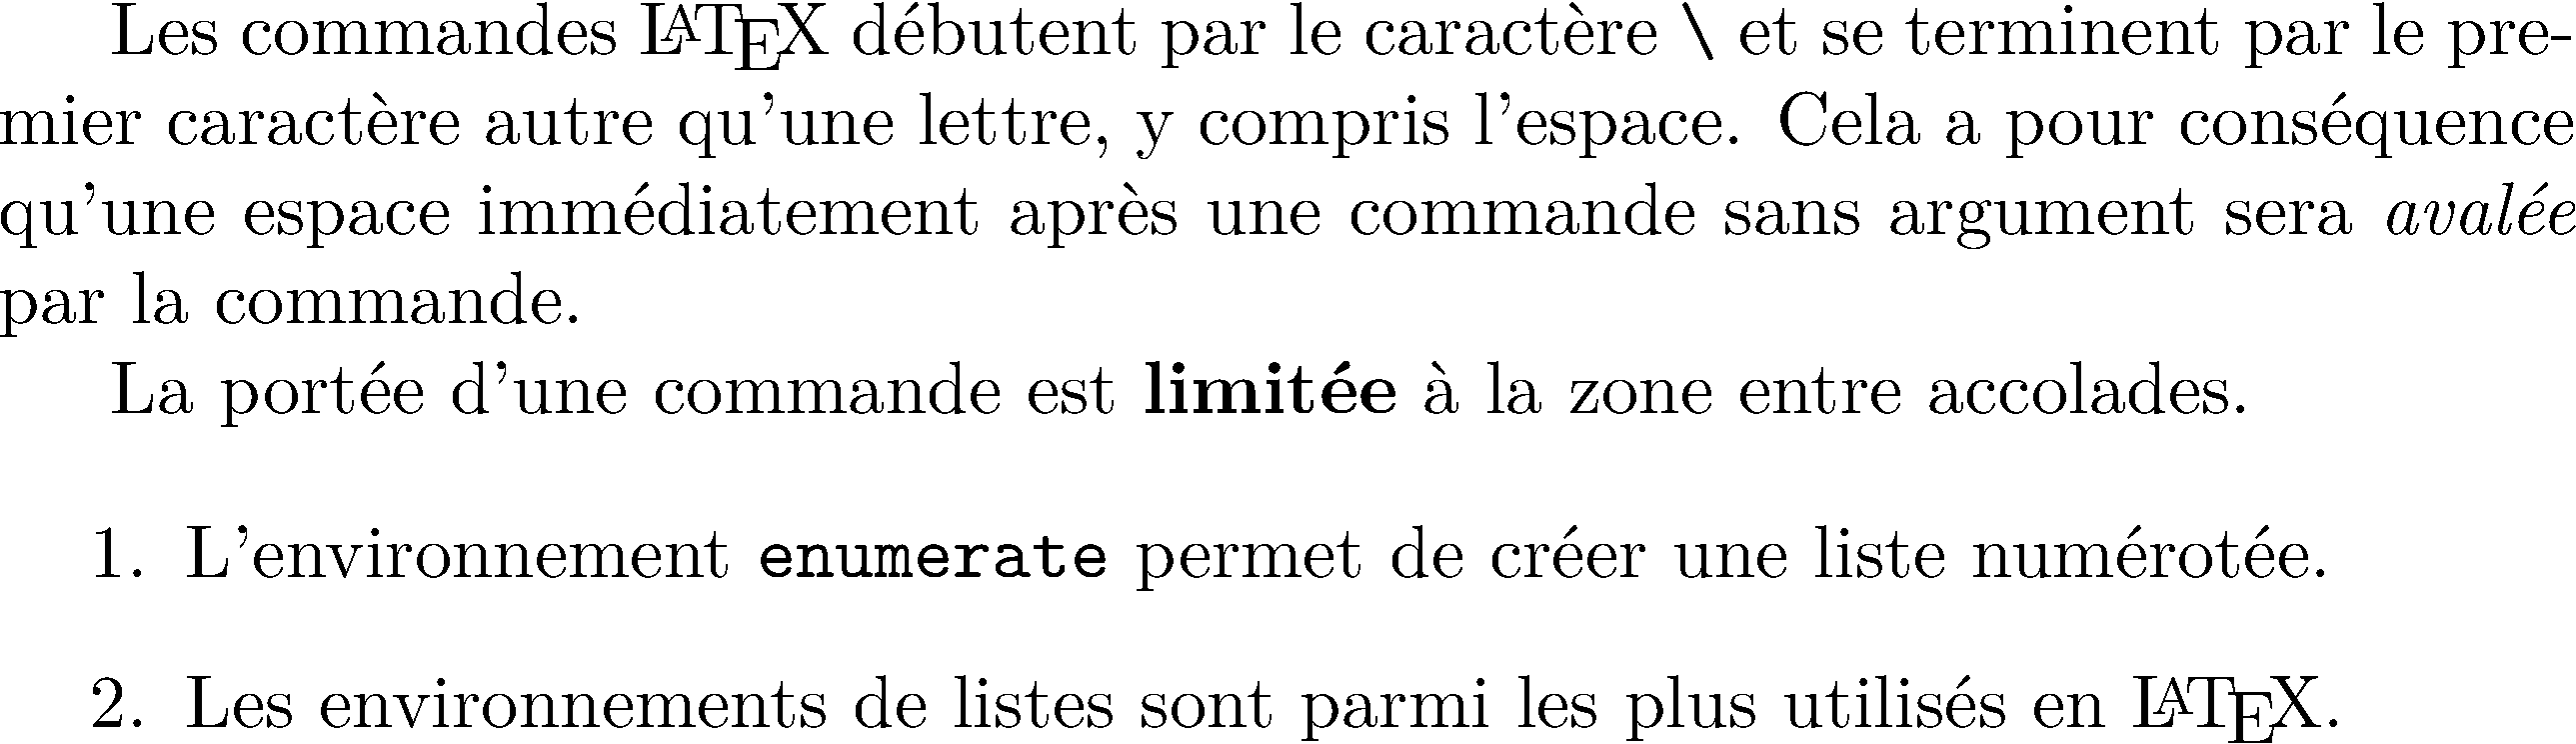
\includegraphics[width=0.95\linewidth]{exercice_commandes-output}}
  \end{center}
\end{frame}
%%% <<<

\begin{frame}[fragile=singleslide]
  \frametitle{Caractères spéciaux}
  \begin{itemize}
  \item Caractères réservés par {\TeX}:
    \begin{quote}
      \verb=# $ & ~ _ ^ % { }=
    \end{quote}
  \item Pour les utiliser, précéder par \verb=\=:
   \begin{quote}
     \begin{minipage}{0.07\linewidth}
\begin{lstlisting}
\#
\end{lstlisting}
      \end{minipage}
      \quad
      \begin{texoutput}{0.07\linewidth}
        \#
      \end{texoutput}
      \hfill
     \begin{minipage}{0.07\linewidth}
\begin{lstlisting}
\$
\end{lstlisting}
     \end{minipage}
     \quad
     \begin{texoutput}{0.07\linewidth}
       \$
     \end{texoutput}
     \hfill
     \begin{minipage}{0.07\linewidth}
\begin{lstlisting}
\%
\end{lstlisting}
     \end{minipage}
     \quad
     \begin{texoutput}{0.07\linewidth}
       \%
     \end{texoutput}
     \\[-0.8\baselineskip]
     \begin{minipage}{0.07\linewidth}
\begin{lstlisting}
\_
\end{lstlisting}
     \end{minipage}
     \quad
     \begin{texoutput}{0.07\linewidth}
       \_
     \end{texoutput}
     \hfill
     \begin{minipage}{0.07\linewidth}
\begin{lstlisting}
\{
\end{lstlisting}
     \end{minipage}
     \quad
     \begin{texoutput}{0.07\linewidth}
       \}
     \end{texoutput}
     \hfill
     \begin{minipage}{0.07\linewidth}
\begin{lstlisting}
\}
\end{lstlisting}
     \end{minipage}
     \quad
     \begin{texoutput}{0.07\linewidth}
       \}
     \end{texoutput}
    \end{quote}
  \item Guillemets:
    \begin{quote}
     \begin{minipage}{0.45\linewidth}
\begin{lstlisting}[escapeinside={}]
``guillemets anglais''
\end{lstlisting}
     \end{minipage}
     \quad
     \begin{texoutput}{0.45\linewidth}
       ``guillemets anglais''
     \end{texoutput}
     \\[-0.8\baselineskip]
     \begin{minipage}{0.45\linewidth}
\begin{lstlisting}
«guillemets français»
\end{lstlisting}
     \end{minipage}
     \quad
     \begin{texoutput}{0.45\linewidth}
       «guillemets français»
     \end{texoutput}
   \end{quote}
  \item Tiret, tiret demi-cadratin, tiret cadratin:
    \begin{quote}
     \begin{minipage}{0.07\linewidth}
\begin{lstlisting}
-
\end{lstlisting}
     \end{minipage}
     \quad
     \begin{texoutput}{0.07\linewidth}
       -
     \end{texoutput}
     \hfill
     \begin{minipage}{0.07\linewidth}
\begin{lstlisting}
--
\end{lstlisting}
     \end{minipage}
     \quad
     \begin{texoutput}{0.07\linewidth}
       --
     \end{texoutput}
     \hfill
     \begin{minipage}{0.07\linewidth}
\begin{lstlisting}
---
\end{lstlisting}
     \end{minipage}
     \quad
     \begin{texoutput}{0.07\linewidth}
       ---
     \end{texoutput}
   \end{quote}
 \end{itemize}
\end{frame}

\begin{frame}[fragile]
  \frametitle{Classe de document}
  \begin{itemize}[<+->]
  \item La première commande du préambule est normalement la
    déclaration de la classe de la forme
\begin{lstlisting}
\documentclass[`\textit{options}']{`\textit{classe}'}
\end{lstlisting}
  \item Principales classes:
    \begin{quote}
      \class{article, report, book, letter} \\
      {\color{emphasis} \class{memoir}} \\
      {\color{emphasis} \class{ulthese}}
    \end{quote}
  \item Principales options:
    \begin{quote}
      \texttt{10pt, {\color{emphasis} 11pt}, 12pt} \\
      \texttt{oneside, twoside} \\
      \texttt{openright, openany} \\
      {\color{emphasis} \texttt{article}} (classe \class{memoir})
    \end{quote}
  \end{itemize}
\end{frame}

\begin{frame}[fragile]
  \frametitle{Paquetages}
  \begin{itemize}
  \item Permettent de modifier des commandes ou d'ajouter des
    fonctionnalités au système
  \item Chargés dans le préambule avec
    \begin{lstlisting}
\usepackage{`\textit{paquetage}'}
\usepackage[`\textit{options}']{`\textit{paquetage}'}
\usepackage{`\textit{paquetage1,paquetage2,...}'}
    \end{lstlisting}
  \item<2-> Les incontournables:
    \begin{description}
      \small
      %% \hfill = PMLA (Poor Man's Left Align) !
    \item[babel*\hfill] typographie multilingue
    \item[inputenc*\hfill] composition en français (\LaTeX)
    \item[fontspec*\hfill] contrôle des polices (\XeLaTeX)
    \item[amsmath\hfill] extensions mathématiques
    \item[booktabs*\hfill] amélioration des tableaux
    \item[hyperref*\hfill] hyperliens dans PDF
    \end{description}
    {\footnotesize * = chargé par défaut dans \class{ulthese}}
  \end{itemize}
\end{frame}

\begin{frame}
  \frametitle{{\LaTeX} en français}
    \small
  \begin{tabularx}{1.0\linewidth}{Xl}
    \toprule
    \textbf{Enjeu} & \textbf{Solution} \\
    \midrule
    \addlinespace[6pt]
    traduction des mots-clés prédéfinis & \pkg{babel} \\
    \addlinespace[6pt]
    coupure de mots & \pkg{babel} \\
    \addlinespace[6pt]
    typographie française & \pkg{babel} \\
    \addlinespace[6pt]
    lettres accentuées dans source & \pkg{inputenc} (\LaTeX) \\
                                   & source en UTF-8 (\XeLaTeX) \\
    \addlinespace[6pt]
    virgule comme séparateur décimal & \pkg{icomma} \\
    \addlinespace[6pt]
    espace comme séparateur des milliers & \pkg{numprint}
  \end{tabularx}
\end{frame}

%%% >>>
\begin{frame}[plain,fragile=singleslide]
  \begin{exercice}
    \begin{enumerate}
    \item Compiler tel que fourni le fichier
      \fichier{exercice\_classe+paquetages.tex}.
    \item Changer la police de caractère du document pour 11~points,
      puis 12~points. Changer la classe du document pour
      \class{memoir}. Observer l'effet sur les marges et sur la
      coupure automatique des mots.
    \item Charger le paquetage \pkg{icomma} et observer l'effet sur
      la formule mathématique.
    \item Charger le paquetage \pkg{numprint} avec l'option
      \verb=autolanguage= (\emph{après} le paquetage \pkg{babel}).
      Dans le code source de la formule mathématique, changer
\begin{lstlisting}
10 000
\end{lstlisting}
      pour
\begin{lstlisting}
\nombre{10000}
\end{lstlisting}
      et observer le résultat.
    \end{enumerate}
  \end{exercice}
\end{frame}
%%% <<<

\section{Parties d'un document}

\begin{frame}[plain]
  \begin{conseil}
    Utiliser impérativement les commandes {\LaTeX} pour identifier
    les différentes parties (la structure) d'un document
  \end{conseil}
\end{frame}

\begin{frame}[fragile]
  \frametitle{Structure logique d'un livre}
  \framesubtitle{(classes \class{book}, \class{memoir}, \class{ulthese})}
\begin{lstlisting}
\frontmatter
\end{lstlisting}
  \begin{itemize}
    \small
  \item préface, table des matières, etc.
  \item numérotation des pages en chiffres romains (i, ii, ...)
  \item chapitres non numérotés
  \end{itemize}
  \vfill

\begin{lstlisting}
\mainmatter
\end{lstlisting}
  \begin{itemize}
    \small
  \item le contenu à proprement parler
  \item numérotation des pages à partir de 1 en chiffres arabes
  \item chapitres numérotés
  \end{itemize}
  \vfill

\begin{lstlisting}
\backmatter
\end{lstlisting}
  \begin{itemize}
    \small
  \item tout le reste (bibliographie, index, etc.)
  \item numérotation des pages se poursuit
  \item chapitres non numérotés
  \end{itemize}
\end{frame}

\begin{frame}[fragile]
  \frametitle{Titre et page titre}
  \begin{itemize}
  \item Mise en forme automatique
    \begin{lstlisting}
%% préambule
\title{`\textit{Titre du document}'}
\author{`\textit{Prénom Nom}'}
\date{`\textit{31 octobre 2014}'} % automatique si omis

%% corps du document
\maketitle
    \end{lstlisting}
  \item Mise en forme libre \\[6pt]
    \begin{minipage}{0.45\linewidth}
      \begin{block}{\small classes standards}
\begin{lstlisting}
\begin{titlepage}
  ...
\end{titlepage}
\end{lstlisting}
      \end{block}

    \end{minipage}
    \hfill
    \begin{minipage}{0.45\linewidth}
      \begin{block}{\small classe \class{memoir}}
\begin{lstlisting}
\begin{titlingpage}
  ...
\end{titlingpage}
\end{lstlisting}
      \end{block}
    \end{minipage}
  \end{itemize}
\end{frame}

\begin{frame}[fragile=singleslide]
  \frametitle{Résumé}
  \begin{itemize}
  \item Classes \class{article}, \class{report} ou \class{memoir}:
    résumé créé avec l'environnement
\begin{lstlisting}
\begin{abstract}

\end{abstract}
\end{lstlisting}
  \item Classe \class{ulthese}: résumés français et anglais traités
    comme des chapitres normaux (non numérotés)
  \end{itemize}
\end{frame}

\begin{frame}[fragile]
  \frametitle{Table des matières}
  \begin{itemize}
  \item Table des matières produite automatiquement avec
\begin{lstlisting}
\tableofcontents
\end{lstlisting}
  \item Requiert plusieurs compilations
  \item Sections non numérotées pas incluses
  \item Avec \pkg{hyperref}, produit également la table des
    matières du fichier PDF
  \item<2-> Classe \class{memoir} fournit également
\begin{lstlisting}
\tableofcontents*
\end{lstlisting}
    qui n'insère pas la table des matières dans la table des matières
  \item<3-> Aussi disponibles:
\begin{lstlisting}
\listoffigures
\listoftables
\end{lstlisting}
    (et leurs versions \verb=*= dans \class{memoir})
  \end{itemize}
\end{frame}

\begin{frame}[fragile=singleslide]
  \frametitle{Sections}
  \begin{itemize}
  \item Découpage du document en sections avec les commandes
    \begin{quote}
      \begin{tabularx}{1.0\linewidth}{Xl}
        \verb=\part= \\
        \verb=\chapter= \\
        \verb=\section= \\
        \verb=\subsection= \\
        \verb=\subsubsection= &
          \color{emphasis} \faArrowLeft\ à éviter dans un livre! \\
        \verb=\paragraph=  &
          \color{emphasis} \faArrowLeft\ jamais (?) utilisé \\
      \end{tabularx}
    \end{quote}
  \item Prennent le titre en argument
  \item Numérotation automatique
  \item Commande suivie d'une \verb=*= = section non numérotée
  \end{itemize}
\end{frame}

\begin{frame}[fragile=singleslide]
  \frametitle{Annexes}
  \begin{itemize}
  \item Annexes sont des sections ou chapitres avec une numérotation
    alphanumérique (A, A.1, ...)
  \item Prochaines sections identifiées comme des annexes par la
    commande
\begin{lstlisting}
\appendix
\end{lstlisting}
  \item Dans le titre, «Chapitre» changé pour «Annexe» le cas échéant
  \end{itemize}
\end{frame}

%%% >>>
\begin{frame}[fragile=singleslide,plain]
  \begin{exercice}
    Utiliser le fichier \fichier{exercice\_parties.tex}.
    \begin{enumerate}
    \item Étudier la structure du document dans le code source.
    \item Ajouter un titre et un auteur au document.
    \item Créer la table des matières du document en le compilant 2 à
      3 fois.
    \item Insérer deux ou trois titres de sections de différents niveaux
      dans le document.
    \item Vous remarquerez que la numérotation cesse à partir des
      sous-sections. C'est une particularité de la classe
      \class{memoir}.

      Recompiler le document après avoir ajouté au préambule la commande
\begin{lstlisting}
\maxsecnumdepth{subsection}
\end{lstlisting}
    \item Ajouter une annexe au document.
    \end{enumerate}
  \end{exercice}
\end{frame}
%%% <<<


\section{Renvois automatiques}

\begin{frame}[fragile=singleslide]
  \frametitle{Parce que l'ordinateur le fera mieux que vous}
  \begin{itemize}
  \item Ne \alert{jamais} renvoyer manuellement à un numéro de
    section, d'équation, de tableau, etc.
  \item «Nommer» un élément avec \verb=\label=
  \item Faire référence par son nom avec \verb=\ref=
  \item Requiert 2 à 3 compilations
  \end{itemize}
\end{frame}

\begin{frame}[plain,fragile=singleslide]
  \begin{lstlisting}[emph={\label,\ref}]
\section{Définitions}
\label{sec:definitions}

Lorem ipsum dolor sit amet, consectetur
adipiscing elit. Duis in auctor dui. Vestibulum

\section{Historique}

Tel que vu à la section \ref{sec:definitions},
on a...
\end{lstlisting}
  \fbox{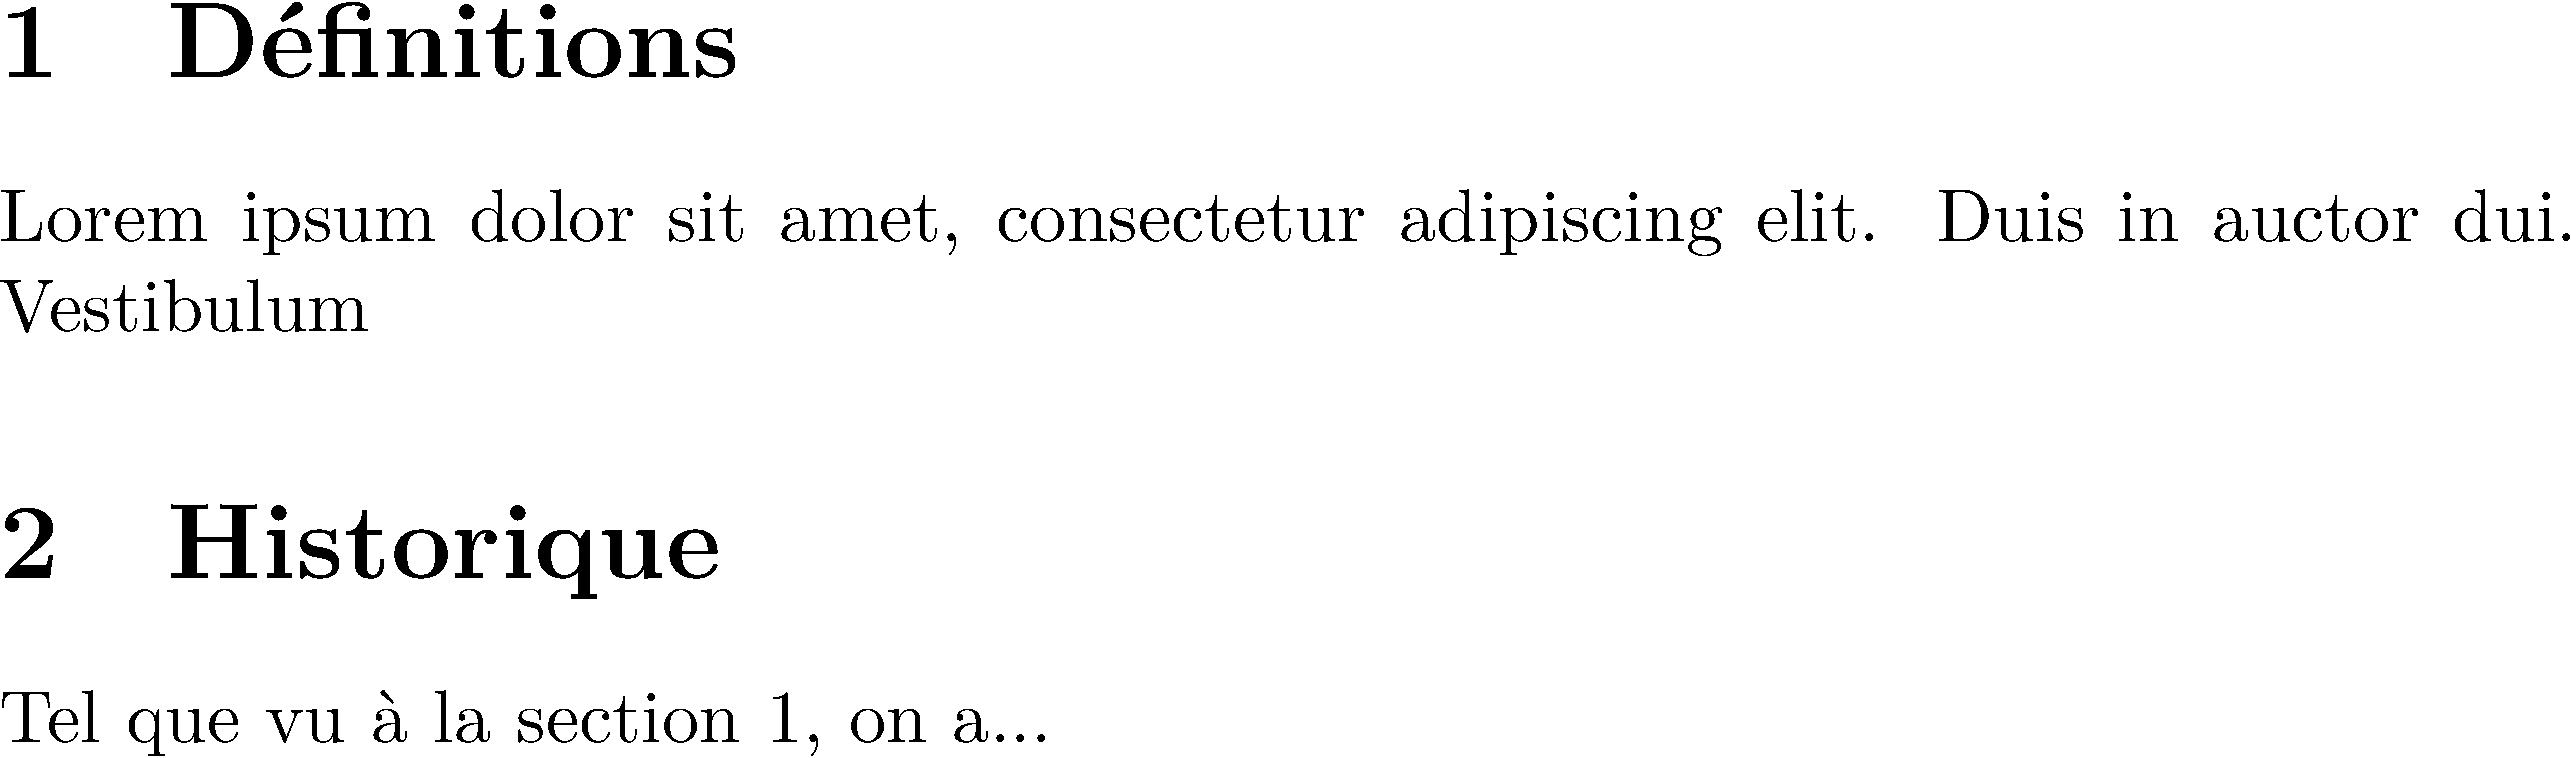
\includegraphics[width=\linewidth]{renvoi}}
\end{frame}

\begin{frame}[plain,fragile=singleslide]
  \begin{conseil}
    Adopter une manière systématique et mnémotechnique de nommer les
    éléments dans un long document afin de vous y retrouver.

    \bigskip %
    Exemple:
\begin{lstlisting}
\label{chap:`\textit{chapitre}'}         % chapitre
\label{sec:`\textit{chapitre}':`\textit{section}'}  % section
\label{tab:`\textit{chapitre}':`\textit{tableau}'}  % tableau
\label{eq:`\textit{chapitre}':`\textit{equation}'}  % équation
\end{lstlisting}
  \end{conseil}
\end{frame}

\begin{frame}[fragile]
  \frametitle{Renvois automatiques++}
  \begin{itemize}
  \item Paquetage \pkg{hyperref} insère des hyperliens vers les
    renvois dans les fichiers PDF
\begin{lstlisting}
Tel que vu à la section \ref{sec:definitions},
on a...
\end{lstlisting}
  \fbox{
\includegraphics[width=0.7\linewidth]{renvoi_avec_ref}}
  \vfill
  \item<2-> Commande \verb=\autoref= permet de
    \begin{enumerate}
    \item nommer automatiquement le type de renvoi (section, équation,
      tableau, etc.)
    \item transformer en hyperlien le texte \textbf{et} le numéro
    \end{enumerate}
\begin{lstlisting}
Tel que vu à la \autoref{sec:definitions},
on a...
\end{lstlisting}
  \fbox{
\includegraphics[width=0.7\linewidth]{renvoi_avec_autoref}}
  \end{itemize}
\end{frame}

%%% >>>
\begin{frame}[plain]
  \begin{exercice}
    Utiliser le fichier \fichier{exercice\_renvois.tex}.
    \begin{enumerate}
    \item Insérer dans le texte un renvoi au numéro d'une section.
    \item Activer le paquetage \pkg{hyperref} avec l'option
      \texttt{colorlinks} et comparer l'effet d'utiliser
      \texttt{{\textbackslash}ref} ou \texttt{{\textbackslash}autoref}
      pour le renvoi.
    \end{enumerate}
  \end{exercice}
\end{frame}
%%% <<<


\section{Apparence du texte}

\begin{frame}
  \frametitle{Police de caractère}
  \begin{itemize}
  \item Par défaut, tous les documents {\LaTeX} utilisent la même
    police de caractère, {\fontfamily{cmr}\selectfont Computer Modern}
  \item Aujourd'hui plus facile d'utiliser d'autres polices, surtout
    avec {\XeLaTeX}
    \begin{itemize}
    \item voir les fichiers d'exercices et les gabarits de
      \class{ulthese} pour des exemples
    \end{itemize}
  \item Privilégier les polices de grande qualité et très complètes
    (lettres accentuées, grand choix de symboles)
    \begin{itemize}
    \item polices Postscript standards ou leurs clones du projet
      TeX~Gyre
    \end{itemize}
  \item Peu de polices sont adaptées pour les mathématiques
    \begin{itemize}
    \item {\fontfamily{ppl}\selectfont Palatino},
      {\fontfamily{ptm}\selectfont Times}, \textrm{Lucida} (\$) sont des choix sûrs
    \end{itemize}
  \end{itemize}
\end{frame}

\begin{frame}[fragile]
  \frametitle{Changement d'attribut de la police de caractères}
  \begin{block}{famille}
    \vspace{-12pt}
    \begin{tabbing}
      \textsf{sans empattements} \qquad\= \verb=\sffamily= \qquad\=
      \verb=\textsf{texte}= \kill
      \small
      \textrm{romain} \> \verb=\rmfamily= \> \verb=\textrm{=\textit{texte}\verb=}= \\
      \texttt{largeur fixe} \> \verb=\ttfamily= \> \verb=\texttt{=\textit{texte}\verb=}= \\
      \textsf{sans empattements} \> \verb=\sffamily= \> \verb=\textsf{=\textit{texte}\verb=}=
    \end{tabbing}
  \end{block}
  \vfill
  \begin{block}{forme}
    \vspace{-12pt}
    \begin{tabbing}
      \textsf{sans empattements} \qquad\= \verb=\sffamily= \qquad\=
      \verb=\textsf{texte}= \kill
      \small
      \textup{\rmfamily droit} \> \verb=\upshape= \> \verb=\textup{=\textit{texte}\verb=}= \\
      \textit{\rmfamily italique} \> \verb=\itshape= \> \verb=\textit{=\textit{texte}\verb=}= \\
      \textsl{penché} \> \verb=\slshape= \> \verb=\textsl{=\textit{texte}\verb=}= \\
      \textsc{\rmfamily petites capitales} \> \verb=\scshape= \> \verb=\textsc{=\textit{texte}\verb=}=
    \end{tabbing}
  \end{block}
  \vfill
  \begin{block}{série}
    \vspace{-12pt}
    \begin{tabbing}
      \textsf{sans empattements} \qquad\= \verb=\sffamily= \qquad\=
      \verb=\textsf{texte}= \kill
      \rmfamily\small
      \textmd{\rmfamily moyen} \> \verb=\mdseries= \> \verb=\textmd{=\textit{texte}\verb=}= \\
      \textbf{\rmfamily gras} \> \verb=\bfseries= \> \verb=\textbf{=\textit{texte}\verb=}= \\
    \end{tabbing}
    \vfill
  \end{block}
  \begin{picture}(0,0)
    \thicklines\color{blue}
    \put(113,30){\dashbox{2}(62,190){}}
    \put(100,20){
      \begin{minipage}[t]{75\unitlength}
        \footnotesize\centering
        s'applique à tout le texte qui suit
      \end{minipage}}
  \end{picture}
  \begin{picture}(0,0)
    \thicklines\color{blue}
    \put(185,30){\dashbox{2}(82,190){}}
    \put(180,20){
      \begin{minipage}[t]{85\unitlength}
        \footnotesize\centering
        s'applique au texte en argument
      \end{minipage}}
  \end{picture}
\end{frame}

\begin{frame}[fragile]
  \frametitle{Taille de la police}
  \vspace{-2pt}
  \begin{block}{commandes standards}
    \vspace{-10pt}
    \begin{tabbing}
      \verb=\footnotesize= \quad\= \kill
      \verb=\tiny= \> {\tiny minuscule} \\
      \verb=\scriptsize= \> {\scriptsize très petit} \\
      \verb=\footnotesize= \> {\footnotesize plus petit} \\
      \verb=\small= \> {\small petit} \\
      \verb=\normalsize= \> {\normalsize normal} \\
      \verb=\large= \> {\large grand} \\
      \verb=\Large= \> {\Large plus grand} \\
      \verb=\LARGE= \> {\LARGE un peu plus grand} \\
      \verb=\huge= \> {\huge encore plus grand} \\
      \verb=\Huge= \> {\Huge énorme}
    \end{tabbing}
  \end{block}
  \vspace{-10pt}
  \pause
  \begin{block}{ajouts de \class{memoir} (et donc \class{ulthese})}
    \vspace{-10pt}
    \begin{tabbing}
      \verb=\footnotesize= \quad\= \kill
      \verb=\miniscule= \quad\> [$<$ \verb=\tiny=] \\
      \verb=\HUGE= \> [$>$ \verb=\Huge=] \\
    \end{tabbing}
  \end{block}
\end{frame}

\begin{frame}[fragile]
  \frametitle{Emphase}
  \begin{itemize}
  \item<1-> Une des propriétés les \emph{plus utilisées} dans le texte
  \item<1-> Commande spécifique:
\begin{lstlisting}
\emph{`\textit{texte}'}
\end{lstlisting}
    \vfill
  \item<2-> Par défaut: texte en italique dans texte droit et vice versa

\begin{lstlisting}
C'était un peu \emph{rough} par moments
\end{lstlisting}
    \begin{texoutput}{\textwidth}
      C'était un peu \emph{rough} par moments
    \end{texoutput}

\begin{lstlisting}
Il m'a dit: «\emph{C'était un peu \emph{rough}
par moments}»
\end{lstlisting}
    \begin{texoutput}{\textwidth}
      Il m'a dit: «\emph{C'était un peu \emph{rough} par moments}»
    \end{texoutput}
    \vfill
  \item<3-> Pas de commande pour souligner en {\LaTeX\dots} et ce n'est
    pas une omission!
  \end{itemize}
\end{frame}


\section{Portions de texte spéciales}

\begin{frame}[fragile=singleslide]
  \frametitle{Listes}
  \begin{itemize}
  \item Deux principales sortes de listes:
    \begin{enumerate}
    \item \alert{à puce} avec environnement \verb=itemize=
    \item \alert{numérotée} avec environnement \verb=enumerate=
    \end{enumerate}
  \item Possible de les imbriquer les unes dans les autres
  \item Marqueurs alors adaptés automatiquement
  \end{itemize}
\end{frame}

\begin{frame}[fragile]
  \frametitle{Code de la diapositive précédente}
\begin{lstlisting}
\begin{itemize}
\item Deux principales sortes de listes:
  \begin{enumerate}
  \item à puce avec environnement \verb=itemize=
  \item numérotée avec environnement \verb=enumerate=
  \end{enumerate}
\item Possible de les imbriquer les unes
  dans les autres
\item Marqueurs adaptés automatiquement
\end{itemize}
\end{lstlisting}
\end{frame}

\begin{frame}[fragile]
  \frametitle{Puce par défaut en français}
  \begin{itemize}
  \item Mode français de \pkg{babel} redéfinit la puce de 1{\ier}
    niveau par défaut de {\textbullet} à {\textemdash}
  \item Pour changer, utiliser dans le préambule
\begin{lstlisting}
\frenchbsetup{
  ItemLabeli=\`\textit{commande}',
  ItemLabelii=\`\textit{commande}'}
\end{lstlisting}
  \item Voir les ressources pour une vaste sélection de symboles
  \end{itemize}
\end{frame}

\begin{frame}[fragile=singleslide]
  \frametitle{Texte centré}
  \begin{center}
    Pour obtenir du texte centré on utilise l'environnement
    \verb=center=
  \end{center}

\begin{lstlisting}
\begin{center}
  Pour obtenir du texte centré on utilise
  l'environnement \verb=center=
\end{center}
\end{lstlisting}

\centering ou encore la commande \verb=\centering=

\begin{lstlisting}
\centering ou encore la commande \verb=\centering=
\end{lstlisting}
\end{frame}

\begin{frame}[fragile=singleslide]
  \frametitle{Citations}
  Deux environnements de citation dans {\LaTeX} (et \class{ulthese})
  \begin{enumerate}
  \item \verb=quote= pour les citations courtes, quelques lignes seulement
    \begin{itemize}
    \item retrait à gauche et à droite
    \end{itemize}
  \item \verb=quotation= pour les citations plus longues se comptant
    en paragraphes
    \begin{itemize}
    \item retrait à gauche et à droite
    \item gestion des marques de paragraphes
    \end{itemize}
  \end{enumerate}
\end{frame}

\begin{frame}[fragile]
  \frametitle{Notes de bas de page}
  \begin{itemize}
  \item Note de bas de page insérée avec la commande
\begin{lstlisting}
\footnote{`\textit{texte de la note}'}
\end{lstlisting}
  \item Commande doit suivre immédiatement le texte à annoter
  \item Méthode recommandée
\begin{lstlisting}[emph=footnote]
... fera remarquer que Pierre Lasou\footnote{%
  Spécialiste en ressources documentaires} %
fut d'une grande aide dans la préparation de ...
\end{lstlisting}
  \item Numérotation et disposition automatiques
  \end{itemize}
\end{frame}

\begin{frame}[fragile=singleslide]
  \frametitle{Code source}
  \begin{itemize}
  \item Environnement \verb=verbatim=
\begin{lstlisting}
\begin{verbatim}
Texte disposé exactement tel qu'il est tapé
dans une police à largeur fixe
\end{verbatim}
\end{lstlisting}
  \item Commande \verb=\verb= dont la syntaxe est
\begin{lstlisting}
\verb`\textit{c}' `\textit{source}' `\textit{c}'
\end{lstlisting}
    où \textit{c} est un caractère quelconque ne se trouvant pas dans
    \textit{source}
  \item Pour usage plus intensif, voir le paquetage \pkg{listings}
  \end{itemize}
\end{frame}

%%% >>>
\begin{frame}[plain]
  \begin{exercice}
    \begin{enumerate}
    \item Ouvrir le fichier \fichier{exercice\_complet.tex} et en
      étudier le code source, puis le compiler.
    \item En comparant le résultat avec le fichier produit avec le
      fichier \fichier{exercice\_tdm+annexes.tex}, déterminer l'effet
      de l'option \texttt{article} dans la classe.
    \item Effectuer les modifications suivantes au document.
      \begin{enumerate}[a)]
      \item Dernier paragraphe de la première section, placer toute la
        phrase débutant par \texttt{«De simple dérivé»} à l'intérieur
        d'une commande \texttt{{\textbackslash}emph}.
      \item Changer la puce des listes pour le caractère
        \texttt{\$>\$}.
      \end{enumerate}
    \end{enumerate}
  \end{exercice}
\end{frame}
%%% <<<



\section{B.a.-ba du mode mathématique}

\begin{frame}[fragile=singleslide]
  \frametitle{Préliminaires}
  \begin{itemize}
  \item Décrire des équations mathématiques requiert un «langage» spécial
    \begin{itemize}
    \item il faut informer {\LaTeX} que l'on passe à ce langage
    \item par le biais de modes mathématiques
    \end{itemize}
  \item Important d'utiliser un mode mathématique
    \begin{itemize}
    \item règles de typographie spéciales (constantes vs variables,
      disposition des équations, numérotation, etc.)
    \item espaces entre les symboles et autour des opérateurs gérées
      automatiquement
    \end{itemize}
  \item Vous voulez utiliser le paquetage \pkg{amsmath}
\begin{lstlisting}
\usepackage{amsmath}
\end{lstlisting}
    \begin{itemize}
    \item lire la documentation de ce paquetage pour connaître toutes
      ses fonctionnalités
    \end{itemize}
  \end{itemize}
\end{frame}

\begin{frame}[fragile]
  \frametitle{Modes mathématiques}
  \begin{enumerate}[<+->]
  \item «En ligne» directement dans le texte comme $(a + b)^2 = a^2 +
    2ab + b^2$ en plaçant l'équation entre \verb=$ $=
\begin{lstlisting}
«En ligne» directement dans le texte
comme $(a + b)^2 = a^2 + 2ab + b^2$
\end{lstlisting}
  \item «Hors paragraphe» séparé du texte principal comme
    \begin{displaymath}
      \int_0^\infty f(x)\, dx = \sum_{i = 1}^n \alpha_i e^{x_i} f(x_i)
    \end{displaymath}
    en utilisant divers types d'environnements
\begin{lstlisting}
«Hors paragraphe» séparé du texte principal comme
\begin{displaymath}
  \int_0^\infty f(x)\, dx =
  \sum_{i = 1}^n \alpha_i e^{x_i} f(x_i)
\end{displaymath}
\end{lstlisting}
  \end{enumerate}
\end{frame}

\begin{frame}[plain]
  \begin{conseil}
    Les équations, en ligne ou hors paragraphe, font partie intégrante
    de la phrase.

    \bigskip %
    Les règles de ponctuation usuelles s'appliquent donc aux
    équations.
  \end{conseil}

  \vspace{18pt}
  \fbox{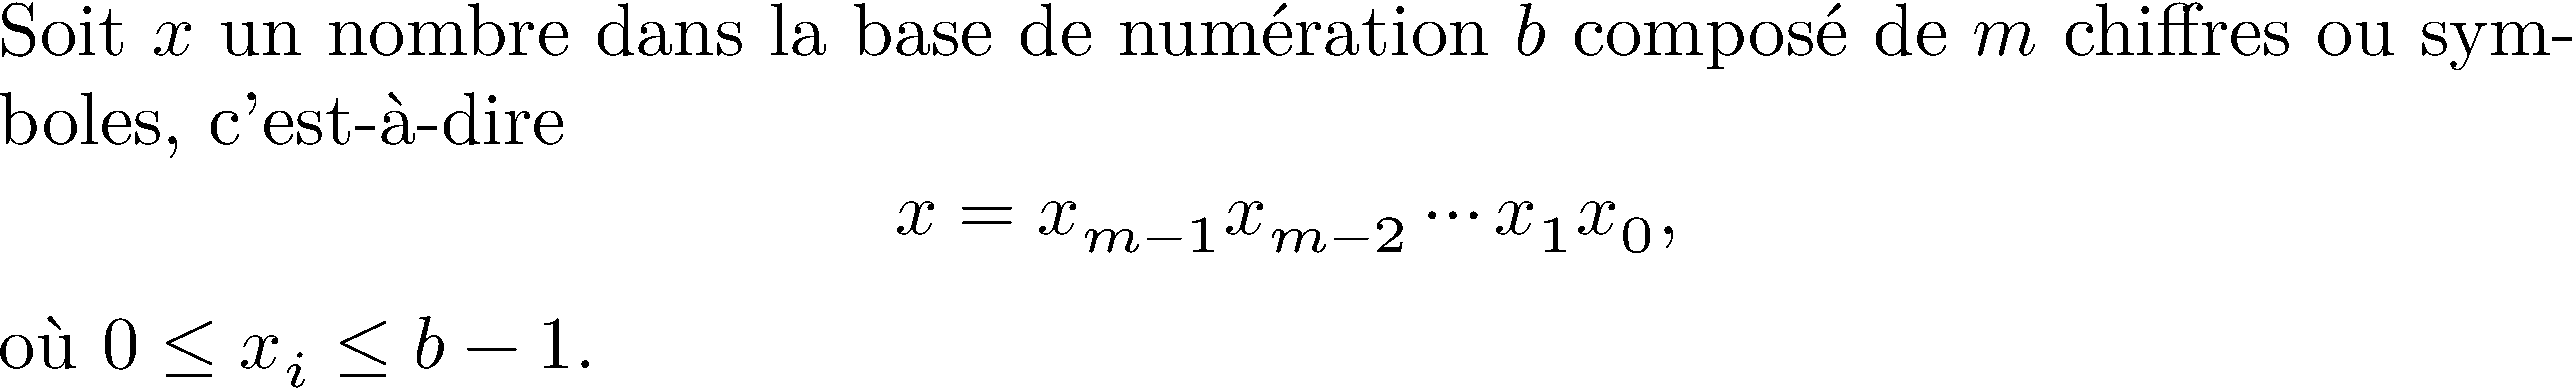
\includegraphics[width=0.95\linewidth]{ponctuation}}
\end{frame}

\begin{frame}[fragile]
  \frametitle{Quelques règles de base}
  \begin{itemize}
  \item En mode mathématique, {\TeX} respecte automatiquement la
    convention d'écrire les constantes en \rmfamily{romain} et les
    variables en \textit{italique}
    \begin{quote}
      \begin{minipage}{0.45\linewidth}
\begin{lstlisting}
$z = 2a + 3y$
\end{lstlisting}
      \end{minipage}
      \hfill
      \begin{texoutput}{0.45\linewidth}
        $z = 2a + 3y$
      \end{texoutput}
    \end{quote}
  \item Espace entre les éléments géré automatiquement, peu importe le
    code source
\begin{quote}
      \begin{minipage}{0.45\linewidth}
\begin{lstlisting}
$z=2 a+3 y$
\end{lstlisting}
      \end{minipage}
      \hfill
      \begin{texoutput}{0.45\linewidth}
        $z=2 a+3 y$
      \end{texoutput}
    \end{quote}
  \end{itemize}
\end{frame}

\begin{frame}[fragile]
  \frametitle{Quelques règles de base (suite)}
  \begin{itemize}
  \item \alert{Ne pas} utiliser le mode mathématique pour obtenir du
    texte en italique!
    \begin{quote}
      \begin{minipage}{0.45\linewidth}
\begin{lstlisting}
\emph{xyz}
\end{lstlisting}
      \end{minipage}
      \hfill
      \begin{texoutput}{0.45\linewidth}
        \rmfamily\emph{xyz}
      \end{texoutput} \\
      \begin{minipage}{0.45\linewidth}
\begin{lstlisting}
$xyz$
\end{lstlisting}
      \end{minipage}
      \hfill
      \begin{texoutput}{0.45\linewidth}
        $xyz$
      \end{texoutput}
    \end{quote}
  \item Utiliser la commande \verb=\text{}= de \pkg{amsmath} pour
    obtenir du texte à l'intérieur du mode mathématique
\begin{quote}
      \begin{minipage}{0.55\linewidth}
\begin{lstlisting}
$x = 0 \text{ si } y < 2$
\end{lstlisting}
      \end{minipage}
      \hfill
      \begin{texoutput}{0.35\linewidth}
          $x = 0 \text{ si } y < 2$
      \end{texoutput}
    \end{quote}
  \end{itemize}
\end{frame}

% \begin{frame}[fragile]
%   \frametitle{Exposants et indices}
%   \begin{itemize}
%   \item Utiliser \verb=^= pour mettre le caractère suivant en exposant
%   \item Utiliser \verb=_= pour mettre le caractère suivant en indice
%   \item Pour plus d'un caractère, regrouper entre \verb={ }=
%   \item Toutes les combinaisons possibles
%   \end{itemize}
%   \pause
%   \begin{quote}
%     \begin{minipage}{0.2\linewidth}
% \begin{lstlisting}
% $x^2$
% \end{lstlisting}
%     \end{minipage}
%     \quad
%     \begin{texoutput}{0.2\linewidth}
%         $x^2$
%       \end{texoutput}
%     \hfill
%     \begin{minipage}{0.2\linewidth}
% \begin{lstlisting}
% $x_4$
% \end{lstlisting}
%     \end{minipage}
%     \quad
%     \begin{texoutput}{0.2\linewidth}
%       $x_4$
%     \end{texoutput}
%     \\
%     \begin{minipage}{0.2\linewidth}
% \begin{lstlisting}
% $x^{2n}$
% \end{lstlisting}
%     \end{minipage}
%     \quad
%     \begin{texoutput}{0.2\linewidth}
%       $x^{2n}$
%     \end{texoutput}
%     \hfill
%     \begin{minipage}{0.2\linewidth}
% \begin{lstlisting}
% $x^{y^2}$
% \end{lstlisting}
%     \end{minipage}
%     \quad
%     \begin{texoutput}{0.2\linewidth}
%       $x^{y^2}$
%     \end{texoutput}
%     \\
%     \begin{minipage}{0.5\linewidth}
% \begin{lstlisting}
% $A_{j_{(k, l)}}^{x_i^2}$
% \end{lstlisting}
%     \end{minipage}
%     \quad
%     \begin{texoutput}{0.3\linewidth}
%       $A_{j_{(k, l)}}^{x_i^2}$
%     \end{texoutput}
%   \end{quote}
% \end{frame}

% \begin{frame}[fragile]
%   \frametitle{Fractions}
%   \begin{itemize}
%   \item Pour les équations en ligne, utiliser tout simplement la barre
%     oblique \verb=/=
%     \begin{quote}
%       \begin{minipage}{0.5\linewidth}
% \begin{lstlisting}
% On a $y = (n + m)/2$.
% \end{lstlisting}
%       \end{minipage}
%       \quad
%       \begin{texoutput}{0.4\linewidth}
%         \rmfamily On a $y = (n + m)/2$.
%       \end{texoutput}
%     \end{quote}
%   \item Pour écrire le numérateur au-dessus du dénominateur, utiliser
%     la commande \verb=\frac{}{}=
%     \begin{quote}
%       \begin{minipage}{0.75\linewidth}
% \begin{lstlisting}
% $\frac{x}{2}$
% \end{lstlisting}
%       \end{minipage}
%       \quad
%       \begin{texoutput}{0.15\linewidth}
%         $\dfrac{x}{2}$
%       \end{texoutput}
%       \\
%       \begin{minipage}{0.75\linewidth}
% \begin{lstlisting}
% $\frac{x_i + \frac{1}{2}}{y^2 + k}$
% \end{lstlisting}
%       \end{minipage}
%       \quad
%       \begin{texoutput}{0.15\linewidth}
%         $\dfrac{x_i + \frac{1}{2}}{y^2 + k}$
%       \end{texoutput}
%     \end{quote}
%   \end{itemize}
% \end{frame}

% \begin{frame}[fragile]
%   \frametitle{Lettres grecques \\ et autres symboles mathématiques}

%   La plupart des symboles mathématiques sont invoqués par une commande
%   dont le nom correspond au nom ou à la signification mathématique du
%   symbole

%   \begin{quote}
%     \begin{minipage}{0.55\linewidth}
% \begin{lstlisting}
% $\mu + \sigma^2 + \gamma$
% \end{lstlisting}
%     \end{minipage}
%     \quad
%     \begin{texoutput}{0.35\linewidth}
%       $\mu + \sigma^2 + \gamma$
%     \end{texoutput}
%     \\
%     \begin{minipage}{0.55\linewidth}
% \begin{lstlisting}
% $\Lambda + \Delta + \Gamma$
% \end{lstlisting}
%     \end{minipage}
%     \quad
%     \begin{texoutput}{0.35\linewidth}
%       $\Lambda + \Delta + \Gamma$
%     \end{texoutput}
%     \\
%     \begin{minipage}{0.55\linewidth}
% \begin{lstlisting}
% $\times \div \leq \geq \neq$
% \end{lstlisting}
%     \end{minipage}
%     \quad
%     \begin{texoutput}{0.35\linewidth}
%       $\times \div \leq \geq \neq$
%     \end{texoutput}
%     \\
%     \begin{minipage}{0.55\linewidth}
% \begin{lstlisting}
% $\dots \cdots \cdot$
% \end{lstlisting}
%     \end{minipage}
%     \quad
%     \begin{texoutput}{0.35\linewidth}
%       $\cdot \dots \cdots$
%     \end{texoutput}
%     \\
%     \begin{minipage}{0.71\linewidth}
% \begin{lstlisting}
% $\sum_{x = 0}^\infty \int_0^x y\, dy$
% \end{lstlisting}
%     \end{minipage}
%     \quad
%     \begin{texoutput}{0.15\linewidth}
%       $\displaystyle \sum_{x = 0}^\infty \int_0^x y\, dy$
%     \end{texoutput}
%   \end{quote}
% \end{frame}

\begin{frame}[fragile=singleslide]
  \frametitle{Environnements pour les équations hors paragraphe}
  \begin{itemize}
  \item Équations d'une seule ligne \newline
    \begin{quote}
      \begin{minipage}[t]{0.4\linewidth}
        \begin{block}{numérotées}
\begin{lstlisting}
equation
\end{lstlisting}
        \end{block}
      \end{minipage}
      \hfill
      \begin{minipage}[t]{0.4\linewidth}
        \begin{block}{non numérotées}
\begin{lstlisting}
displaymath
equation*
\end{lstlisting}
        \end{block}
      \end{minipage}
    \end{quote}
  \item Séries d'équations alignées, généralement sur \verb|=|
    \begin{quote}
      \begin{minipage}[t]{0.4\linewidth}
        \begin{block}{numérotées}
\begin{lstlisting}
align
\end{lstlisting}
        \end{block}
      \end{minipage}
      \hfill
      \begin{minipage}[t]{0.4\linewidth}
        \begin{block}{non numérotées}
\begin{lstlisting}
align*
\end{lstlisting}
        \end{block}
      \end{minipage}
    \end{quote}
  \end{itemize}
\end{frame}

\begin{frame}[fragile]
  \frametitle{Avant-goût}

  Pouvez-vous interpréter ce code?
\begin{lstlisting}
\begin{displaymath}
  \Gamma(\alpha) =
  \sum_{j = 0}^\infty \int_j^{j + 1}
    x^{\alpha - 1} e^{-x}\, dx
\end{displaymath}
\end{lstlisting}
  \vspace{18pt}
  \pause

  Fort probablement!
  \begin{displaymath}
    \Gamma(\alpha) =
    \sum_{j = 0}^\infty \int_j^{j + 1} x^{\alpha - 1} e^{-x}\, dx
  \end{displaymath}
\end{frame}


\section{Classe ulthese}

\begin{frame}
  \frametitle{Un document conforme en un tournemain}
  \begin{itemize}
  \item \class{ulthese} livrée dans {\TeX}~Live donc déjà
    installée sur votre ordinateur
  \item Mise en page conforme aux règles de présentation de la FESP
  \item Basée sur la classe \class{memoir}, donc les fonctionnalités
    de celle-ci sont disponibles dans \class{ulthese}
  \item Quelques nouvelles commandes pour la création de la page titre
  \item Partir d'un gabarit (classés avec la documentation dans
    {\TeX}~Live)
  \item Utiliser des fichiers séparés pour chaque chapitre du mémoire
    ou de la thèse
  \end{itemize}
\end{frame}

%%% >>>
\begin{frame}[plain,fragile=singleslide]
  \begin{exercice}
    Utiliser le fichier \fichier{exercice\_ulthese.tex} --- qui est
    basé sur le gabarit \fichier{gabarit-doctorat.tex} livré avec
    \class{ulthese}.
    \begin{enumerate}
    \item Étudier le code source du fichier.

      Remarquer que le fichier \fichier{mathematiques.tex} est inséré
      dans le document avec la commande \verb=\include=. Étudier
      brièvement le code source de ce fichier.
    \item Activer les paquetages \pkg{amsmath} et \pkg{icomma},
      puis compiler \fichier{exercice\_ulthese.tex}.
    \item Modifier un environnement \texttt{align*} pour
      \texttt{align} dans \fichier{mathematiques.tex} et observer le
      résultat dans la compilation de \fichier{exercice\_ulthese.tex}.
    \item Compiler de nouveau le fichier en utilisant une police de
      caractères différente.
    \end{enumerate}
  \end{exercice}
\end{frame}
%%% <<<


\section{Ressources}

\begin{frame}
  \frametitle{Quelques essentiels}
  \begin{itemize}
  \item Un excellent livre de référence
    \begin{quote}
      \href{http://ariane.ulaval.ca/cgi-bin/recherche.cgi?qu=a1982705}{%
        \emph{Guide to {\LaTeX}}, 4{\ieme} éd., de H.~Kopka et P.W.~Daly}
    \end{quote}
  \item En français, en ligne, libre
    \begin{quote}
      \href{http://fr.wikibooks.org/wiki/LaTeX}{%
        \emph{LaTeX} dans Wikilivre}
    \end{quote}
  \item Foire aux questions bien garnie
    \begin{quote}
      \href{http://www.tex.ac.uk/cgi-bin/texfaq2html}{%
        \emph{UK List of {\TeX} Frequently Asked Questions}}
    \end{quote}
  \item Forum de discussion très actif
    \begin{quote}
      \href{http://tex.stackexchange.com}{%
        {\TeX}--{\LaTeX} Stack Exchange}
    \end{quote}
  \item Liste de symboles disponibles dans {\LaTeX}
    \begin{quote}
      \href{http://www.ctan.org/tex-archive/info/symbols/comprehensive/}{%
        \emph{The Comprehensive {\LaTeX} Symbol List}} \\
      (aussi fournie avec {\TeX}~Live)
    \end{quote}
  \end{itemize}
\end{frame}

{
  \setbeamercolor{background canvas}{bg=black}

  \begin{frame}[plain]
    \advance\textwidth-10mm
    \hsize\textwidth
    \columnwidth\textwidth %
    \scriptsize\color{lightgray} %
    \vfill
    \begin{center}
      \begin{minipage}{0.7\textwidth}
        \raggedright %
        Ce document a été produit avec le système de mise en page
        {\XeLaTeX} à partir de la classe \textbf{beamer}. Le texte
        principal est en Lucida Sans~OT, le code informatique en
        Lucida Grande Mono~DK et les titres en Adobe Myriad~Pro. Les
        icônes proviennent de la police Font~Awesome.
      \end{minipage}
    \end{center}
    \vfill
  \end{frame}
}

%%% Local Variables:
%%% mode: latex
%%% TeX-master: "formation_latex_UL-partie_1"
%%% End:


\end{document}

%%% Local Variables:
%%% TeX-engine: xetex
%%% mode: latex
%%% TeX-master: t
%%% End:
